\chapter{Vortex shedding -- von Karman instability}

\modinfo{Directory}{VonKarmanGUI}
\modinfo{Solvers}{\Idx{FlowSolve}}
\modinfo{Tools}{\Idx{ElmerGUI}}
\modinfo{Dimensions}{2D, Transient}
\modinfo{Author}{Peter R{\aa}back}

\subsection*{Case definition}

%\begin{flushleft}
This tutorial is about simulating the developing of the
vortex shedding i.e. the von Karman instability. 
The geometry is a tube with a circular obstacle. 
For more details on the problem look at the benckmark case definition by
by M. Sch�fer and S. Turek in \textit{"Benchmark computations of laminar flow around a cylinder"}.


\subsection*{Solution procedure}

The mesh is given in 2d netgen format in file \texttt{circle\_in\_channel.in2d}, load this file.
\ttbegin
File 
  Open -> circle_in_channel.in2d
\ttend
You should get a mesh consisting of 749 nodes and 1328 triangles. This
is a rather sparse mesh. To increase the element number 
\ttbegin
Mesh 
 Configure
   nglib / Max H: 0.02
Mesh 
  Remesh
\ttend
This mesh includes 3464 nodes and 6506 triangles. The mesh is presented in figure~\ref{fg:vonkarman_mesh}.

\begin{figure}[h]
\centering
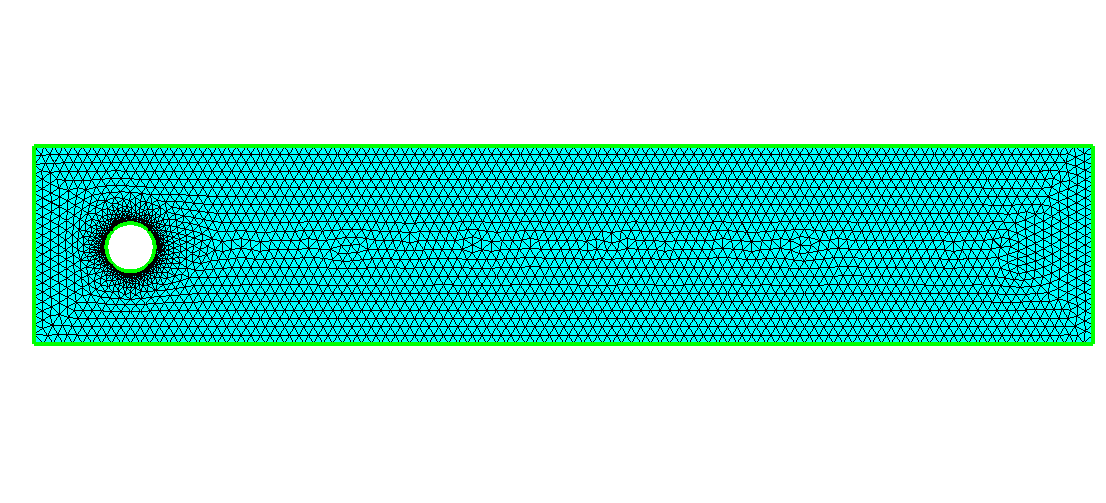
\includegraphics[width=150 mm, height=55 mm]{vonkarman_mesh}
\caption{Computational mesh of the problem.}\label{fg:vonkarman_mesh}
\end{figure}  


After we have the mesh we start to go through the Model menu from the top to bottom. 
In the Setup we choose things related to the whole simulation such as file names, 
time stepping, constants etc.
The simulation is carried out in 2-dimensional cartesian
coordinates. 2nd order bdf time-stepping method is selected with 200 steps
and we want the total simulation time to be 8 seconds. 
\ttbegin
Model
  Setup 
    Simulation Type = Transient
    Steady state max. iter = 1
    Time Stepping Method = bdf
    BDF Order = 2
    Time Step Intervals = 200
    Time Step Sizes = $ 8/200
\ttend
For the solver specific settings we are quite happy to use the defaults. However, we relax a little bit the 
convergence tolerances to get speedier simulation.
\ttbegin
Model
  Equation
    Name = Navier-Stokes
    Apply to Bodies = 1
    Navier-Stokes 
      Active = on
    Edit Solver Settings
      Nonlinear system 
        Convergence tol. = 1.0e-4
      Linear System 
        Convergence tol. = 1.0e-6
    Add 
    OK
\ttend        
The Material section includes all the material parameters.
Here we choose simple parameters for the academic test case
\ttbegin
Model
  Material
    Name = Ideal
    General 
      Density = 1
    Navier Stokes
      Viscosity = 0.001 
    Apply to Bodies = 1 
    Add
    OK
\ttend

The system does not need any body forces. We are also happy with the default initial condition 
of zero and therefore no initial conditions are applied either. Any other initial condition would
require the values to be explicitely set.

We have three different kinds of boundaries: inlet, no-slip walls, and outlet. The inlet
has a parabolic fully developed laminar profile with a maximum velocity of 1.5~m/s.
Additionally for the inlet the vertical velocity component is assumed zero. 
The circle and the lower and upper walls are given the no-slip treatment.
For the outlet only the vertical component is set to zero since the default discretization
weakly imposes a zero pressure condition if the normal velocity component is not defined.
\ttbegin
Model
  BoundaryCondition
    Name = Inlet
    Navier-Stokes 
      Velocity 1 = Variable Coordinate 2; Real MATC "4*1.5*tx*(0.41-tx)/0.41^2"
      Velocity 2 = 0.0
    Add
    New

    Name = Walls
    Navier-Stokes 
      Velocity 1 = 0.0
      Velocity 2 = 0.0
    Add
    New

    Name = Outlet
    Navier-Stokes 
      Velocity 2 = 0.0
    Add 
    Ok
\ttend   

The conditions may also be assigned to boundaries in the Boundary condition menu, or 
by clicking with the mouse. Here we use the latter approach as that spares us of the 
need to know the indexes of each boundary.
\ttbegin
Model
  Set boundary properties
    Choose inlet -> set boundary condition Inlet
    Choose both horizontal walls and circle -> set boundary condition Walls
    Choose outlet -> set boundary condition Outlet
\ttend


For the execution 
ElmerSolver needs the mesh files and the command file. We have now basically defined
all the information for ElmerGUI to write the command file. After writing it we may also visually 
inspect the command file.
\ttbegin
Sif 
  Generate
  Edit -> look how your command file came out  
\ttend

Before we can execute the solver we should save the files in a directory. The project includes
all the files needed to restart the case.
\ttbegin
File 
  Save Project
\ttend

After we have successfully saved the files we may start the solver
\ttbegin
Run
  Start solver
\ttend
A convergence view automatically pops up showing relative changes of each iteration.
The norm after the first timestep should be around 0.695, and after last 0.749, respectively.

When there are some results to view we may start the postprocessor also
\ttbegin
Run
  Start ParaView
\ttend


\subsection*{Results}

Due to the number of the time-steps the simulation will take a few minutes.
You may inspect the results with Paraiew as the time-steps are computed, or
wait until all timesteps have been computed.
You need to reload the files if number of timesteps are increased.

In Figure \ref{fg:vonkarman_flow} the velocity field is presented for three different timesteps.
The maximum velocity in the system should be about 2.1724~m/s. Note that here
visualization was not performed with Paraview and may therefore look quite different.

\begin{figure}[h]
\centering
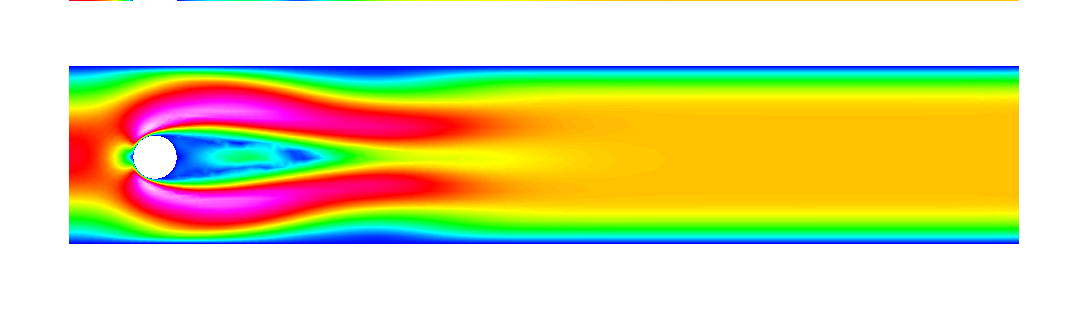
\includegraphics[width=12cm, viewport=0 30 1089 270,clip]{flow20.png}
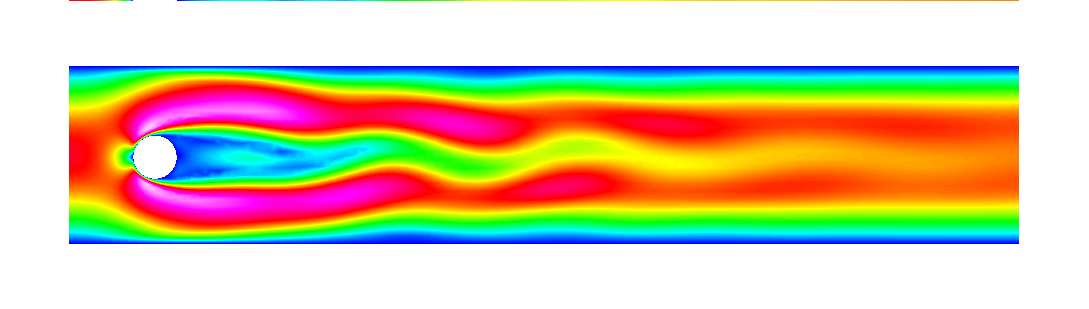
\includegraphics[width=12cm, viewport=0 30 1089 270,clip]{flow100.png}
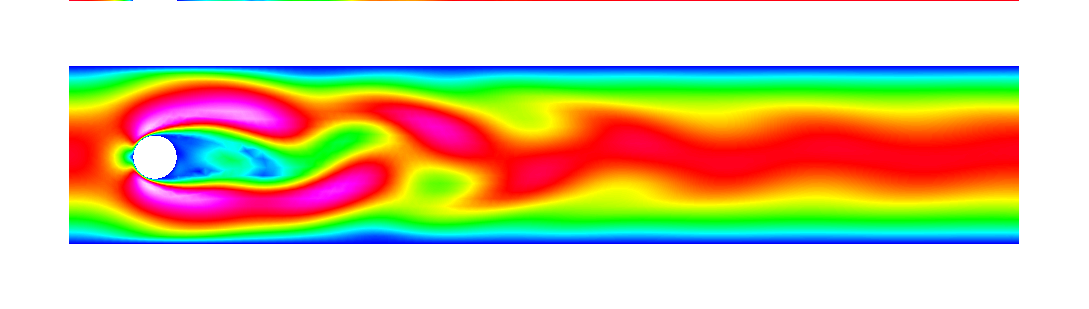
\includegraphics[width=12cm, viewport=0 30 1089 270,clip]{flow200.png}
\caption{Velocity distribution at steps 20, 100 and 200}\label{fg:vonkarman_flow}
\end{figure} 


\subsection*{Effect of Reynolds number}
The Reynolds number in this case is around 100 resulting to unsteady flow.
The critical Reynolds number is around 90 and 
reducing the flow velocity so that Reynolds number becomes, say 20, makes the 
system to possess a steady-state solution. On the other hand, increasing the velocity will make the von Karman vortecis
even more pronounced until they break into fully chaotic motion. This finite element mesh will allow only 
minor increase in Reynolds number to be able to capture the phenomena. 

\hfill

